This exercise relates to the \say{Hwk-data1} dataset, which can be found in Canvas.

\nl Operators of gasoline-fueled vehicles complain about the price of gasoline in gas stations. According to
the American Petroleum Institute, the federal gas tax per gallon is constant (18.4 cents as of January
13, 2005), but state and local taxes vary from 7.5 cents to 32.10 cents for $n = 18$ key metropolitan areas
around the country.

\nl \textit{Use R for part (a), (b), and (c)}

\begin{enumerate}
    \item Check whether the data are normally distributed by using the Shapiro test or by looking at the QQ
plot. (Make sure to display your results).

\noindent 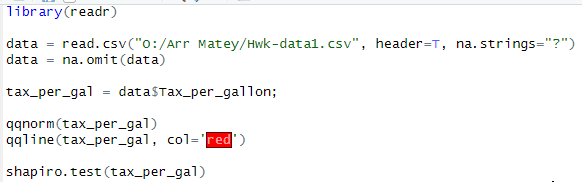
\includegraphics[width=5in]{r_2a-1.PNG}

\noindent 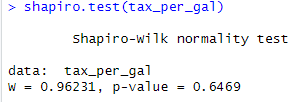
\includegraphics[width=3in]{r_2a-3.PNG}

\noindent Since $p = 0.6469 > \alpha$ (assuming $\alpha = 0.05$), the data are normally distributed.

\noindent 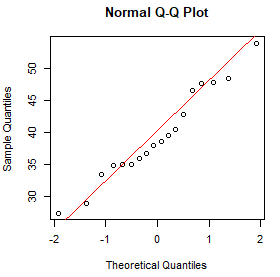
\includegraphics[width=3.5in]{r_2a-2.PNG}\newpage
    \item Use the appropriate R function to find a 90\% confidence interval for the average per gallon gas tax in
the U.S. (Make sure to display your code and the corresponding result.)

\noindent 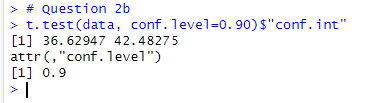
\includegraphics[width=3.5in]{r_2b.PNG}

\noindent The confidence interval $I := (36.62947, 42.48275)$.\vspace{0.3in}
    \item Is there sufficient evidence to claim that the average gas tax is less that 45.2 cents? (Make sure to
specify hypotheses and the p-value).

\soln* $H_0 := \mu = 45.2$ and $H_a := \mu < 45.2$.

\noindent 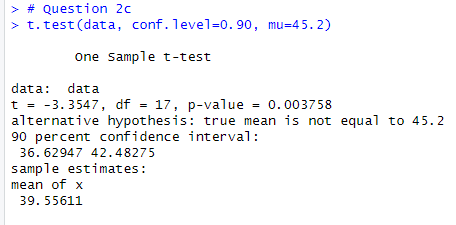
\includegraphics[width=3.5in]{r_2c.PNG}

\noindent Since $p =0.003758 \leq 0.1 = \alpha$, we reject the null hypothesis ($H_0$). Hence, there is sufficient evidence that the true mean of the gas tax is less than 45.2 cents.\vspace{0.3in}
    \item Compute (by hand) a 98\% confidence interval for the average per gallon gas tax in the U.S. Compare
the length of this interval and the one in part (b). (Hint: the sample standard deviation $s = 7.138$)

\soln* $\Xbar \approx 39.556$, $\df = 18-1 = 17$, and $\alpha = 0.02$. Then $t_{\alpha/2}(17) = t_{0.01}(17) = 2.567$.

\nl Then the CI is $39.556 \pm 2.567 \pfrac{7.138}{\sqrt{18}} \equiv (35.237, 43.875)$. The measure of this interval is $8.638$ cents, whereas in part (b) the measure was $5.85328$ cents. Higher confidence levels require more of the domain since $\lim_{\alpha \to 0^+} \equiv D$. 
\end{enumerate}